\documentclass{amsart}
\setcounter{tocdepth}{2}

\usepackage{amsfonts, amsthm, mathtools}
\usepackage{xcolor}
\usepackage{graphicx}
\usepackage{tikz-cd}
\usepackage{stmaryrd}
\usepackage[margin=1in]{geometry}
\usepackage{setspace}
\DeclareMathOperator{\Emb}{Emb}
% \dim is already defined as a math operator by amsmath.
% \DeclareMathOperator{\dim}{dim}
\DeclareMathOperator{\Mfd}{Mfd}
\DeclareMathOperator{\Hom}{Hom}
\DeclareMathOperator{\red}{red}
\DeclareMathOperator{\Map}{Map}
\DeclareMathOperator{\Man}{Man}
\DeclareMathOperator{\Disc}{Disc}
\DeclareMathOperator{\Psh}{PSh}
\DeclareMathOperator{\Diff}{Diff}
\DeclareMathOperator{\Top}{Top}
\DeclareMathOperator{\BTop}{BTop}
\DeclareMathOperator{\BO}{BO}
\DeclareMathOperator{\GL}{GL}
\DeclareMathOperator{\nc}{nc\mathcal{B}ord}

\DeclareMathOperator{\conf}{conf}
\DeclareMathOperator{\FR}{FR}
\DeclareMathOperator{\TM}{TM}
\onehalfspacing
\raggedbottom

% Theorem environments
\newtheorem{theorem}{Theorem}[section]
\newtheorem{lemma}[theorem]{Lemma}
\newtheorem{corollary}[theorem]{Corollary}
\newtheorem{proposition}[theorem]{Proposition}
\theoremstyle{definition}
\newtheorem{definition}[theorem]{Definition}
\theoremstyle{remark}
\newtheorem{remark}[theorem]{Remark}
\theoremstyle{example}
\newtheorem{example}[theorem]{Example}

% TO DO

\begin{document}

\title{Kleine AT III, Embedding Calculus: Talk I}
\date{\today}


\maketitle

\tableofcontents

\section{The Space of Embeddings}

For the space of embeddings of $M \hookrightarrow N$, we use the following notation
\[
\Emb^o(M, N)
\]
to denote the space of smooth embeddings, topologized as a subspace of smooth maps $C^{\infty}(M,N)$ in the smooth topology. We use $t$ instead of $o$ to denotes topological embeddings, \textcolor{red}{and omit the superscript when talking about both??? We will maybe omit this superscript lets see}. For the purpose of this talk, we will restrict to the case where $\dim(M) = \dim(N)$ and denote this dimension $d$ (because we want to eventually build the category $\Mfd_d$). We stick to discussing mostly the smooth case.

\subsection{Motivation}

If we care about understanding manifolds, we care about embedding spaces. Manifolds can be understood by embeddings into them (we will come back to this idea later), while their diffeomorphism groups can be given by letting diffeomorphisms act on embeddings. This is explained via the isotopy extension theorem, which  allows us to extend an isotopy between two embeddings of a manifold inside another one to a diffeomorphism of the ambient manifold. Recall that an \textbf{isotopy} is a homotopy $H \colon I \to \Emb(M, N)$ from one embedding $e_0 \in  \Emb^o(M,N)$ to another $e_1 \in \Emb^o(M,N)$, such that $H(t)$ is an embedding for all $t$. Extending this to a diffeomorphism of $N$, (or rather to an ambient isotopy) means finding a lift $\widetilde H:I\to\operatorname{Diff}(N)$ of $H$ with $\widetilde H(0)=\operatorname{id}_N$.
\begin{equation}\label{eq:isotopy-extension-diagram}
\begin{tikzcd}[row sep=large, column sep=large]
    & \Diff(N) \arrow[d, "F"] \\
    I \arrow[r, "H"'] \arrow[ur, dotted, "\widetilde H"] & \Emb(M,N)
\end{tikzcd}
\end{equation}
where the map $F$ is defined by letting a diffeomorphism act on our initial embedding $e_0 \in \Emb^o(M,N)$:
    \[
    \begin{aligned}
        F \colon \Diff(N) &\to \Emb^o(M,N) \\
        \varphi &\mapsto \varphi \circ e_0
    \end{aligned}
    \]
We can imagine an isotopy $H$ extending to a diffeomorphism of $N$ as such:

\begin{center}
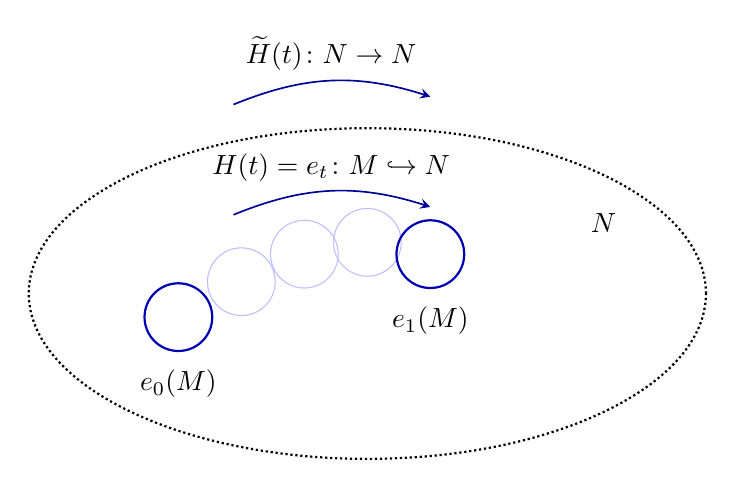
\begin{tikzpicture}[x=1cm,y=1cm]
    % The dotted outline represents the ambient manifold schematically.
    \draw[densely dotted, thick] (0,0) ellipse (4.3 and 2.1);
    \node at (3,0.9) {$N$};

    % Faint snapshots of the moving embedded copy of M.
    \foreach \x/\y in {-1.6/0.15,-0.8/0.5,0/0.65} {
        \draw[blue!25, thin] (\x,\y) circle (0.43);
    }
    \draw[blue!70!black, thick] (-2.4,-0.3) circle (0.43);
    \draw[blue!70!black, thick] (0.8,0.5) circle (0.43);
    \node[below] at (-2.4,-0.85) {$e_0(M)$};
    \node[below] at (0.8,-0.05) {$e_1(M)$};

    \draw[->, >=stealth, blue!60!black, semithick]
        (-1.7,1) to[bend left=20]
        node[above, text=black] {$H(t)=e_t\colon M\hookrightarrow N$} (0.8,1.1);
    % The ambient isotopy acts on all of N.
    \draw[->, >=stealth, blue!60!black, semithick]
        (-1.7,2.4) to[bend left=20]
        node[above, text=black] {$\widetilde H(t)\colon N\to N$} (0.8,2.5);
\end{tikzpicture}
\par\smallskip
\refstepcounter{figure}\label{fig:ambient-isotopy}
Figure~\thefigure
\end{center}

In fact, our isotopy extension theorem says something stronger; that under certain conditions our map $F$ is a fibration.

\begin{theorem}[Isotopy Extension Theorem]
    Need citation! Let $M$ be compact and $N$ have no boundary. Fix an embedding $e_0 \colon M \hookrightarrow N$. Then the map
    \[
    \begin{aligned}
        F \colon \Diff(N) &\to \Emb^o(M,N) \\
        \varphi &\mapsto \varphi \circ e_0
    \end{aligned}
    \]
    is a Serre fibration.
\end{theorem}

\begin{remark}
    Note that the homotopy lifting property for $CW-$complexes $X$
    \[
    \begin{tikzcd}[row sep=large, column sep=large]
    X \arrow[d, hook] \arrow[r] & \Diff(N) \arrow[d, "F"] \\
    X \times I \arrow[r, "H"'] \arrow[ur, dotted, "\widetilde H"] & \Emb(M,N)
    \end{tikzcd}
    \]
    when $X = \{ * \}$ is exactly the diagram we had before in~\eqref{eq:isotopy-extension-diagram}.
\end{remark}


\begin{remark}
    The fiber over an embedding $e \in \Emb^o(M,N)$ is non-empty if and only if there exists some diffeomorphism $\varphi \in \Diff(N)$ such that $\varphi \circ e_0 = e$.
\end{remark}

\begin{corollary}
    If the fiber is non-empty, it is given by 
    \[
    F^{-1}(e) = \Diff_{\delta}(N \backslash \overset{\circ}{e(M)})
    \]
    the group of diffeomorphisms of $N$ without the interior of $M$ such that $\Diff(\delta e(M)) = id_{\delta M}$ and all derivatives of the diffeomorphism on the boundary of $M$ agree with derivatives of $id_{\delta M}$. The fiber inclusion is given by extension-by-identity:
    \[
    \begin{aligned}
        \Diff_{\delta}(N \backslash \overset{\circ}{e(M)}) &\hookrightarrow \Diff(N) \\
        f &\to \widetilde{f} = \begin{cases}
            f \text{ on } N \backslash \overset{\circ}{e(M)}\\
            Id \text{ on e(M)}
        \end{cases}
    \end{aligned}
    \]
\end{corollary}

\begin{center}
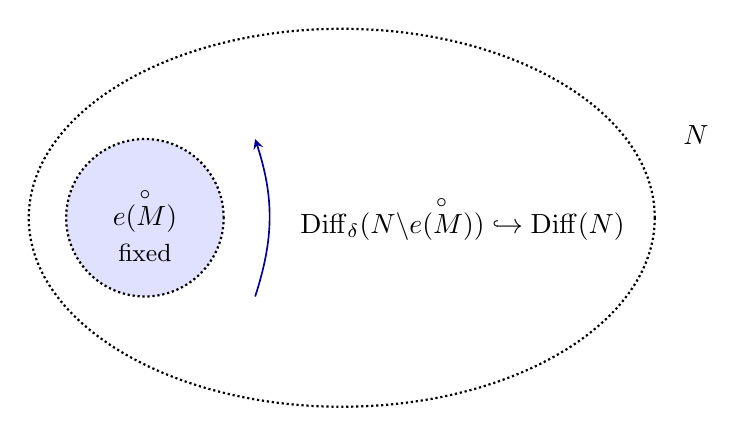
\begin{tikzpicture}[x=1cm,y=1cm]
    % Schematic ambient manifold and the region fixed by extension.
    \draw[densely dotted, thick] (0,0) ellipse (3.975 and 2.4);
    \node at (4.5,1.05) {$N$};
    \begin{scope}[xshift=5mm]
    \fill[blue!12] (-3,0) circle (1);
    \draw[densely dotted, thick] (-3,0) circle (1);
    \node at (-3,0.1) {$\overset{\circ}{e(M)}$};
    \node[font=\small] at (-3,-0.45) {fixed};

    % This arrow suggests the action in the complement, not a point trajectory.
    \draw[->, >=stealth, blue!60!black, semithick]
        (-1.6,-1) to[bend right=18] (-1.6,1);
    \node[anchor=west] at (-1.15,0)
        {$\Diff_{\delta}(N\backslash\overset{\circ}{e(M)})\hookrightarrow\Diff(N)$};
    \end{scope}
\end{tikzpicture}
\par\smallskip
\refstepcounter{figure}\label{fig:extension-by-identity}
Figure~\thefigure
\end{center}



“The fiber sequence resembles $H\to G\to G/H$: the orbit of $e_0$ in the embedding space is the quotient of $\operatorname{Diff}(N)$ by the subgroup fixing $e_0(M)$ pointwise. In this sense, you can rememember the slogan \dots

Slogan: "embedding spaces measure the differences between diffeomorphism groups". Specifically, $\Emb(M,N)$ measures the difference between diffeomorphisms of $N$ and diffeomorphisms of $N$ leaving the embedded manifold $M$ fixed in $N$.

\subsection{Examples}

\begin{example}
    The topological group of diffeomorphisms $\Diff(N) \subset \Emb^o(N,N)$ is the subset of smooth embeddings admitting a strict inverse, i.e.
    \[
    \Diff(N) = \{ \Emb^o(N,N) \ | \ \exists \ e^{-1} \text{ with } e^{-1} \circ e = e \circ e^{-1} = id \}
    \]
    When $N$ is closed, $\Diff(N) = \Emb^o(N,N)$.
\end{example}

\begin{example}
    The inclusions 
    \[
    \GL_d(\mathbb{R}) \hookrightarrow \Diff(\mathbb{R}^d) \hookrightarrow \Emb(\mathbb{R}^d, \mathbb{R}^d)
    \]
    are homotopy equivalences with inverse taking the derivative at the origin.
\end{example}

\begin{example}
    Recall that a framed knot is an embedding $S^1 \times D^2 \hookrightarrow S^3$. $\pi_0(\Emb(S^1 \times D^2, S^3)) = $ the set of framed knots up to isotopy.
\end{example}

Let $\underbar{k} = \{1, \dots, k\}$ be a collection of $k$ points.

\begin{example}
    The space of embeddings of $k$ points in $M$ is the ordered configuration space of $k$ points $\Emb(\underbar{k}, M) \cong \conf_k(M)$.
\end{example}

\begin{example}
    $\Emb(\mathbb{R}^d, M) \cong \FR(\TM)$ gives the frame bundle of the manifold, or the principal bundle associated with the tangent bundle of $M$. \textcolor{red}{learn frame bundle}
\end{example}

\begin{example}
    Embedding spaces of open discs are given by framed ordered configuration spaces $\Emb(\underbar{k} \times \mathbf{R}^d, M) = \conf_k(M) \times \FR(\TM)$.
\end{example}

\section{Embedding Calculus}

\subsection{Motivation: A Pointilistic Viewpoint}

A question embedding calculus seeks to answer is how to distinguish manifolds up to diffeomorphism. While we have homotopy invariants, these distinguish only homotopy type. However, we saw by the homotopy extension theorem that embeddings tell us about diffeomorphism groups. So instead of looking at the homotopy types of the manifolds themselves, we look at the homotopy types of spaces of certain embeddings into them. Some of the simplest manifolds we can embed are collections of points $\underbar{k}$ as defined before. However, ordered configuration spaces are homeomorphism invariants. In order to consider the smooth structure as well, we embed instead a finite collection of open disks, and this is a diffeomorphism invariant:



\[
\begin{array}{r@{\;}c@{\qquad}c@{\qquad}l}
    M\text{ and }N\text{ are} & \text{homotopy invariant}
        & \Rightarrow & M \simeq N \\
    & \cup & & \\
    & \text{homeomorphic}
        & \Rightarrow & \Emb(\underbar{k}, M) \simeq \Emb(\underbar{k}, N) \\
    & \cup & & \\
    & \text{diffeomorphic}
        & \Rightarrow & \Emb(\underbar{k} \times \mathbb{R}^d, M) \simeq \Emb(\underbar{k} \times \mathbb{R}^d, N)
\end{array}
\]

\subsection{The Category $\Mfd_d$}

In order to define the embedding tower, we need to define the infinity category of blabla manifolds. For this, first we need to define the topologically enriched $1-$category of $d-$dimensional manifolds. In this subsection we discuss both smooth and topological manifolds, i.e. $c \in \{o, t\}$ and omit this from notation.

\begin{definition}
    Let $\Man_d$ denote the topologically enriched $1-$category with:
    \begin{itemize}
        \item Objects: (smooth or topological) manifolds $M$ with $\dim M = d$
        \item Mapping spaces: $\Map(M,N) = \Emb(M,N)$ (spaces rather than sets, due to topological enrichment)
        \item Composition: composition of embeddings
    \end{itemize}
\end{definition}

\begin{definition}
    Let $\Mfd_d$ be the $\infty-$category of $d-$dimensional manifolds given by the coherent nerve of $\Man_d$: $\Mfd_d = \mathcal{N}(\Man_d)$.
    \begin{itemize}
        \item Objects: (smooth or topological) manifolds $M$ with $\dim M = d$
        \item $\Hom$: $\Map(M,N) \simeq \Emb(M,N)$
        \item Composition: composition of embeddings
    \end{itemize}
\end{definition}

Note that (homotopy) equivalences in $\Mfd_d$ are \textbf{isotopy equivalences}, since the mapping spaces are embedding spaces and homotopies between morphisms here are paths inside $\Emb(M,N)$, i.e. isotopies of embeddings. Therefore, embedding spaces are isotopy invariant. So, for another manifold $P \in \Mfd_d$, we can add the following in our heirarchy of invariants:


\[
\begin{array}{r@{\;}c@{\qquad}c@{\qquad}l}
    M\text{ and }N\text{ are} & \text{diffeomorphic}
        & \Rightarrow & \Emb(\underbar{k} \times \mathbb{R}^d, M) \simeq \Emb(\underbar{k} \times \mathbb{R}^d, N) \\
    & \cup & & \\
    & \text{equivalent in } \Mfd_d
        & \Rightarrow & \Emb(M, P) \simeq \Emb(N, P)
\end{array}
\]

\subsection{Embedding Calculus Tower: without boundary}

One motivation for embedding calculus was to study diffeomorphism groups; after defining $\Mfd_d$ and seeing that equivalences in this category are isotopy equivalences and embedding spaces are invariant under it, \textcolor{red}{our object of study is}
\[
\Emb(M,N)
\]
and embedding calculus then seeks to approximate this embedding space using information given by embedding finite unions of discs into both $M$ and $N$.
We do this first by defining a presheaf via the Yoneda embedding. Let us associate to a $d-$dimensional manifold $M$, a space-valued presheaf $E_M$:
\[
\begin{aligned}
    y \colon \Mfd_d &\to \Psh(\Mfd_d) \\
    M &\mapsto E_M
\end{aligned}
\]
where $E_M$ is a contravariant functor recovering spaces of embeddings into $M$:
\[
\begin{aligned}
    E_M \colon \Mfd_d^{op} &\to \mathcal{S}\\
    M' &\mapsto \Map_{\Mfd_d}(M',M) = \Emb(M', M) 
\end{aligned}
\]
It is clear that $y$ is just the Yoneda Embedding and the image of $M$ is $E_M$, a representable presheaf. Note that $E_M(\emptyset) = \Emb(\emptyset, M) \simeq *$, so $E_M$ is always a \textbf{reduced presheaf}, i.e. one whose value on the empty set is a single point. Applying the Yoneda Lemma here to the presheaf given by $y(N) = E_N$ in $\Psh(\Mfd_d)$ and $M \in \Mfd_d$, we have a canonical isomorphism:
\[
\begin{aligned}
    \underbrace{\begin{gathered}
        \Emb(M,N) \\
        f
    \end{gathered}}_{E_N(M)}
    &\begin{gathered}
        \xrightarrow{\sim} \\
        \mapsto
    \end{gathered}
    &\underbrace{\begin{gathered}
        \Map_{\Psh(\Mfd_d)}(E_M, E_N) \\
        y(f)
    \end{gathered}}_{\substack{\text{natural transformations} \\ \text{between } E_M \text{ and } E_N}}
\end{aligned}
\]
Then embedding calculus asks "to what extent can we recover embedding disks here"

Then let $\Disc \subset \Mfd_d$ be the full subcategory of objects equivalent to $S \times \mathbb{R}^d$ for some finite set $S$, and let $\Disc_{\leq k} \subset \Disc$ be the full subcategory of such objects such that $|S| \leq k$. Because the image of any manifold under the Yoneda embedding is a reduced presheaf, we can restrict to the categories of reduced presheaves.

\begin{lemma}
    The composition of the Yoneda Embedding with the restriction along $\Disc \xhookrightarrow{i} \Mfd_d$ 
    \[
    Y \colon \Mfd_d \xrightarrow{y} \Psh^{\red}(\Mfd_d) \xrightarrow{i_*} \Psh^{\red}(\Disc)
    \]
    induces the \textbf{embedding calculus approximation}
    \[
    \begin{aligned}
        &\begin{aligned}
            &\Emb(M,N) \\
            &= \Map_{\Mfd_d}(M,N)
        \end{aligned}
        \quad \longrightarrow \qquad
        \begin{aligned}
            &T_{\infty}\Emb(M,N) \\
            &\coloneq  \Map_{\Psh^{\red}(\Disc)}(E_M,E_N)
        \end{aligned}
    \end{aligned}
    \]
    \textcolor{red}{which is just the induced map between their mapping spaces}
\end{lemma}
In further talks, we will see that under certain conditions this map is an equivalence. So we aim to create a tower to help us estimate the right hand side. Note that we have a sequence of inclusions of subcategories
\[
\Disc_{\leq 1} \subset \Disc_{\leq 2} \subset \cdots \subset \Disc_{\leq \infty} = \Disc
\]
with $\Disc$ as the colimit. On presheaves we then have a sequence of restrictions of functors
\[
\Psh^{\red}({\Disc_{\leq 1}}) \leftarrow \Psh^{\red}({\Disc_{\leq 2}}) \leftarrow \cdots \leftarrow \Psh^{\red}({\Disc_{\leq \infty}}) = \Psh^{\red}({\Disc})
\]
with $\Psh^{\red}({\Disc})$ as the limit. This restricts further to a tower of the reduced presheaves. Then we can define 
\[
T_{k} \coloneq T_{k}\Emb(M,N) \coloneq \Map_{\Psh^{\red}(\Disc_{\leq k})}(E_M,E_N)
\]
where we use $T_{k}$ as a shorthand. On mapping spaces we get the following tower of finite approximations 
\[
\begin{tikzcd}[row sep=large, column sep=huge]
    & T_{\infty} \arrow[d] \\
    & \vdots \arrow[d] \\
    & T_{\geq 2} \arrow[d] \\
    \Emb(M,N) \arrow[r] \arrow[ur] \arrow[uuur] & T_{\geq 1}
\end{tikzcd}
\]
\begin{center}
\refstepcounter{figure}\label{fig:embedding-calculus-tower}
Figure~\thefigure
\end{center}
with $T_{\infty} \xrightarrow{\sim} \lim_{k \rightarrow \infty} T_{k}$. 

In further talks, we will see how to compute the stages $T_k$ so we can take the limit and understand $T_{\infty}$, but in this talk we cover the first stage, $T_1 = \Map_{\Psh^{\red}(\Disc_{\leq 1})}(E_M,E_N)$. Right Kan extension identifies $\Psh({\Disc_{= 1}})$, presheaves over objects equivalent to $\mathbb{R}^d$ with $\Psh^{\red}({\Disc_{\leq 1}})$, so we can rewrite $T_1 \simeq \Map_{\Psh^{\red}(\Disc_{= 1})}(E_M,E_N)$, which is easier to understand.

\begin{definition}
    The category $\Disc_{= 1}$ is equivalent to the groupoid with
    \begin{itemize}
        \item A single object
        \item Morphisms $\Emb(\mathbb{R}^d, \mathbb{R}^d) \simeq \begin{cases}
            \GL_d(\mathbb{R}) \simeq O(d) &\text{ for } c = o\\
            \Top(d) &\text{ for } c = t
        \end{cases}$
    \end{itemize}
    i.e., in the smooth case it is the groupoid $\BO(d)$ and in the topological case, $\BTop(d)$.
\end{definition}

Viewing the presheaf categories as functors, they unstraighten to the following fibrations \textcolor{red}{citation for Lurie higher topos theory}
\[
    \Psh({\Disc_{= 1}}) = \begin{cases}
        \mathcal{S}_{/ \BO(d)} &\text{ for } c = o\\
        \mathcal{S}_{/ \BTop(d)} &\text{ for } c = t
    \end{cases}
\]
And under this equivalence
    


\subsection{Alternative formulation: with boundary}

We can do the same construction of the tower for manifolds with boundary and will take the approach due to de Brito and Weiss.

Let us consider the category of (potentially noncompact) $d-$dimensional manifolds with boundary a fixed (potentially noncompact) $d-1-$dimensional manifold $P$. This can also be thought of as the category $\nc(d)_{P,\emptyset}$ of potentially noncompact $d-$dimensional bordisms between $P$ and $\emptyset$. Let $\Disc_{P,\emptyset} \overset{i}{\subset} \nc(d)_{P,\emptyset}$ be the full subcategory of bordisms which are diffeomorphic ($c = o$) or homeomorphic ($c = t$) relative to the boundary (so that on the boundary, we have the identity morphism) to $P \times [0,1) \sqcup S \times \mathbb{R}^d$.

\begin{center}
\refstepcounter{figure}\label{fig:bordism}
\edef\bordismfigurenumber{\thefigure}
\refstepcounter{figure}\label{fig:boundary-collars-and-discs}
\edef\discsfigurenumber{\thefigure}
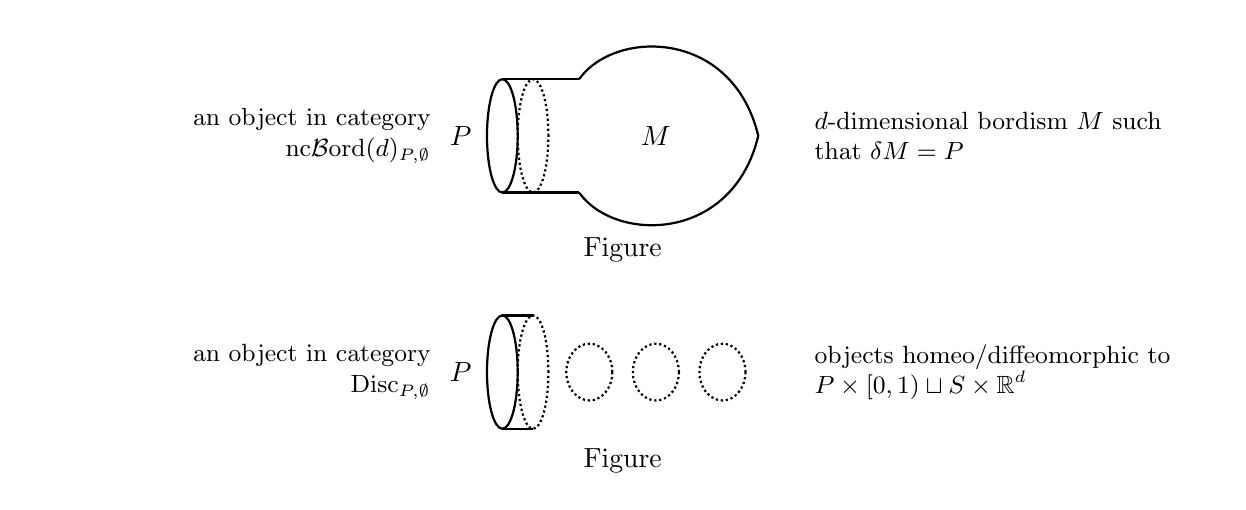
\begin{tikzpicture}[x=0.65cm, y=0.8cm, thick]
    % The bordism, with dotted inner edges of the boundary collars.
    \draw (-3,0) ellipse (0.3 and 0.9);
    \draw (-3,0.9) -- (-1.5,0.9);
    \draw (-3,-0.9) -- (-1.5,-0.9);
    \draw (-1.5,0.9)
        .. controls (-0.8,1.7) and (1.5,1.7) .. (2,0)
        .. controls (1.5,-1.7) and (-0.8,-1.7) .. (-1.5,-0.9);
    \draw[densely dotted] (-2.4,0) ellipse (0.3 and 0.9);
    \node[left] at (-3.4,0) {$P$};
    \node at (0,0) {$M$};
    \node[anchor=east, align=right, text width=5cm, font=\small] at (-4.2,0)
        {\mbox{an object in category}\\$\nc(d)_{P,\emptyset}$};
    \node[anchor=west, align=left, text width=5cm, font=\small] at (2.9,0)
        {$d$-dimensional bordism $M$ such that $\delta M = P$};
    \node at (-0.65,-1.8) {Figure~\bordismfigurenumber};

    % The same boundary collars, together with three interior discs.
    \begin{scope}[yshift=-3cm]
        \draw (-3,0) ellipse (0.3 and 0.9);
        \draw (-3,0.9) -- (-2.4,0.9);
        \draw (-3,-0.9) -- (-2.4,-0.9);
        \draw[densely dotted] (-2.4,0) ellipse (0.3 and 0.9);
        \node[left] at (-3.4,0) {$P$};
        \node[anchor=east, align=right, text width=5cm, font=\small] at (-4.2,0)
            {\mbox{an object in category}\\$\Disc_{P,\emptyset}$};
        \node[anchor=west, align=left, text width=5cm, font=\small] at (2.9,0)
            {objects homeo/diffeomorphic to\\
            \mbox{$P \times [0,1) \sqcup S \times \mathbb{R}^d$}};
        \node at (-0.65,-1.4) {Figure~\discsfigurenumber};
        \foreach \discposition in {-1.3,0,1.3} {
            \draw[densely dotted] (\discposition,0) circle (0.45);
        }
    \end{scope}
\end{tikzpicture}
\end{center}

So instead of embedding just finite collections of disks as we did in the construction with no boundary, we also embed the collar neighborhood corresponding to the boundary of the manifold. Then our Yoneda embedding for the bordism category composed with the restriction along $i$ becomes
\[
\begin{aligned}
    Y \colon \nc(d)_{P,\emptyset} \xrightarrow{y} \Psh(\nc(d)_{P,\emptyset}) \xrightarrow{i_*} \Psh(\Disc_{P,\emptyset}) \\
\end{aligned}
\]
and we filter $\Disc_{P,\emptyset}$ again by the cardinality of our indexing set $S$ and obtain the tower on mapping spaces for manifolds with boundary as before.

To Do 
\begin{enumerate}
    \item straightening unstraightening
    \item right Kan extension
    \item citations
    \item figure out how to get this online
\end{enumerate}

\bibliographystyle{alpha}
\bibliography{referencesAS}

\end{document}
